%% -----------------preamble------------------ %%

%% define the document as an article,
%% size of a4paper, twosided and with two columns
\documentclass[twoside, a4paper, twocolumn]{article}

%% use the utf-8 encoding for the input
\usepackage[utf8]{inputenc}

%% diagrams
\usepackage{pgfplots}
%% set compatibility for version 1.7
\pgfplotsset{compat=1.7}

%% cache diagrams -> faster compile times
\usepgfplotslibrary{external}
\tikzexternalize

%% math env and symbols
\usepackage{amsmath}

%% math more symbols
\usepackage{amssymb}

%% hyperlinks
\usepackage{hyperref}

%% make heading smaller
\usepackage[small]{titlesec}

%% include everything until subsections in the toc
\setcounter{tocdepth}{5}
\setcounter{secnumdepth}{5}
%% ------------------------------------------- %%

\begin{document}
    %% * suffix prints the section without the counter prefix
    \section*{Statistics - Exam preparation}
    %% creates a clickable link, similar to markdown: [xnacly]{https://xnacly.me}
    \href{https://xnacly.me}{xnacly} 
    %% gets replaced with the current date according to your language locale,
    %% for me its: July 19, 2023
    - \today 
    - \href{https://github.com/xnacly/statistics}{source}

    %% creates a table of contents containing all sections,
    %% parts, subsections, subsubsections, paragraphs and subparagraphs
    \tableofcontents

    \section{Introduction}
    Statistics is a fairly big field. Therefore this paper will only include
    the absolutely necessary topics for passing the university class.

    \section{Abstract}
    This paper starts of with symbols used in the field of statistics, their
    meaning and in what context they are commonly used. Following Combinatorics
    is thematized.

    \section{Symbols and special characters}

    %% env to list items, similar to the <ul> HTML tag 
    \begin{itemize}
       %% anything between $ and $ is interpreted as a mathblock
       \item $n!$ Faculty / Fakultät
       \item $\binom{n}{k}$ Binomial Coefficient / Binomialkoeffizient
       \item $\Omega$ Event set / Ergebnismenge
       \item $\omega$ Result / Ergebnis
       \item $A \subseteq \Omega$ Event / Ereignis
       \item $\{\omega\}$ Elementary event / Elementarereignis
       \item $\mathbb{P}$ Probability measure / Wahrscheinlichkeitsmaß
       \item $\mathbb{P}(A)$ Event propability / Wahrscheinlichkeit eines Ereignisses
       \item $\mathbb{E}(X), \mu_x, \mu$ Expected value / Erwartungswert
       \item $\sigma$ Standard deviation / Standardabweichung
       \item $\mathrm{Var}(X), \sigma^2_x$ Variance / Varianz
       \item $\mathrm{Cov}(X,Y), \sigma_{XY}$ Kovarianz von X und Y
       \item $\mathcal{N}(\mu, \sigma^2)$ Normal distribution / Normalverteilung
       \item $\varphi$ Bell curve / Glockenkurve
       \item $\Phi$ Error function / Fehlerintegral
       \item $X$ Random variable / Zufallsvariable
       \item $\mathrm{Z}$ Standard score / standard-normalverteilte
           Zufallsvariable
           \footnote{read more: \href{https://en.wikipedia.org/wiki/Standard_score}{wikipedia}}
       \item $\textrm{Bin}(n, p)$ Binomial distribution / Binomialverteilung
       \item $\textrm{Pois}(\lambda)$ Poisson distribution / Poission-Verteilung
       \item $\textrm{Exp}(\lambda)$ Exponential distribution / Exponentialverteilung
    \end{itemize}

    \section{Combinatorics}
    This chapter will introduce the Binomial Coefficient, Factorials, Pascal's
    triangle and the binomial theorem.

    \subsection{Binomial Coefficient}
    %% italic text
    \textit{n choose k}; used to calculate the Amount of Sets in
    %% \textrm allows for non italic characters in math blocks
    $\{1,\textrm{...},n\}$ with exactly $k$ Elements. $n$ needs to be positive
    and $k$ and $n$ have to meet the following criteria: $n \in \mathbb{N}, 0
    \leq k \leq n$.
    %% mathematics env,
    %% adds a counter to the right of the equation and centers the equation
    \begin{equation}
        \binom{n}{k} = \frac{n!}{k! \cdot (n-k)!}
    \end{equation}
    Choosing $k$ different Numbers from $\{1,\textrm{...},n\}$, there are $n$
    possibilities for the first number, $n-1$ possibilities for the second, and
    so forth. 

    \subsubsection{Example:}
    If we were to calculate how many possibilities there are to choose 3 out of
    6 dishes, we can simply use the above formular:
    \begin{align*}
        \binom{6}{3} = \frac{6!}{3! \cdot (6-3)!} = \frac{720}{3! \cdot 3!} =
        \frac{720}{36} = \underline{\underline{20}}
    \end{align*}

    %% this creates a plot
    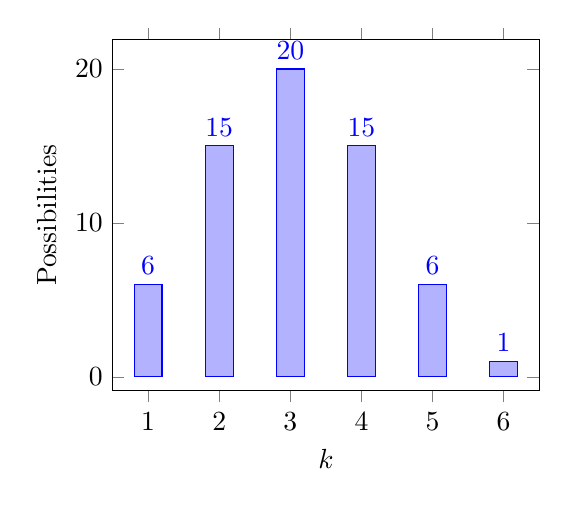
\begin{tikzpicture}
        \begin{axis}[
            %% this adds a label to the x axis
            xlabel=$k$,
            %% this adds a label to the y axis
            ylabel=Possibilities,
            %% only add labels on the x axis if data is at that x value
            xtick=data,
            %% diagram is a bar chart
            ybar,
            %% indicate values of the bars near their ending
            nodes near coords,
            width=7cm,
            ]
            %% add coordinate pairs of one type
            \addplot coordinates {
                (1, 6)
                (2, 15)
                (3, 20)
                (4, 15)
                (5, 6)
                (6, 1)
            };
        \end{axis}
    \end{tikzpicture}

    \subsection{Factorial}
    This can be described with $n!$. The factorial is defined as the
    product of decrementing $n$ by an increasing subtrahend:
    \begin{equation}
        n! := n \cdot (n-1) \cdot (n-2) \textrm{...}
    \end{equation}
    If $n = k$, there are $n!$ possibilities to choose $k$ Elements from $n$.
    $0! = 1$.

    \subsection{Pascal's triangle}
    The pascal's triangle can be used to visualize the binomial
    %% footnotes get displayed at the bottom of the current page and 
    %% are referenced with a superscript number which is a clickable link
    coefficient.\footnote{read more about \textit{pascal's triangle}
    here: \href{https://en.wikipedia.org/wiki/Pascal's_triangle}{wikipedia}}

    \begin{equation}
        \binom{n+1}{k+1} = \binom{n}{k} + \binom{n}{k+1}
    \end{equation}

    \subsection{Binomial Theorem}
    Allows for expressing the exponents of $(x+y)^n, n \in \mathbb{N}$ as a
    polynomial with the degree of $n$.
    \begin{equation}
        (x+y)^n = \sum^n_{k=0} \binom{n}{k} \cdot x^k \cdot y^{n-k}
    \end{equation}

    \section{Probability theory}
    This chapter contains information on how to calculate probabilites.

    \subsection{Event set} The set containing results of the
    \textit{experiment} $E$ is notated via the \textit{event set} ($\Omega$).
    Sub sets of $\Omega$ are \textit{events} ($\omega$). \textit{Events} with
    one entry are \textit{elementary events} $\{\omega\}$. If $\Omega$ is
    finite: $\forall \omega \in \Omega,\mathbb{P}(\omega) \geq 0$. The sum of
    all propabilities of $\omega \in \Omega$ is $1$\footnote{$\sum_{\omega \in
    \Omega} \mathbb{P}(\omega) = 1$}.

    \subsection{Random variable}
    $X: \Omega \rightarrow \mathbb{R}$ we define $\{X = x\} := \{\omega |
    X(\omega) = x\}$ and can therefore shorten our definition of the
    propability that $X$ is $x$ to: $P(X = x) := P(\{X = x\})$
    \begin{eqnarray}
        x \rightarrow \mathbb{P}(X = x) \\
        x \rightarrow \mathbb{P}(X \leq x)
    \end{eqnarray}

    The first equation defines the density / probability function of $X$ and the
    second equation the distribution function of $X$.

    \subsection{Expected value}
    \begin{equation}
        \mathbb{E}(X) = \sum_{k \in \mathbb{R}}k \cdot \mathbb{P}(X = k)
    \end{equation}

    \subsubsection{Example:}
    For a dice:
    %% same as equation, but can be used with & to align equations
    \begin{align*}
        \mathbb{P}(X = k) &= \frac{1}{6}; k = 1,2,3,4,5,6 \\
        \mathbb{E}(X) &= \sum_{k \in 1}^6 k \cdot \mathbb{P}(X = k) \\
                      &= \sum_{k = 1}^6 k \cdot \frac{1}{6} \\
                      &= \frac{1}{6} (1+2+3+4+5+6) \\
                      &= \left\lfloor\frac{21}{6}\right\rfloor =
                      \left\lfloor\frac{7}{2}\right\rfloor = \underline{\underline{3}}
    \end{align*}
    As shown above the expected value is $\frac{7}{2} \approx 3,5$.

    \subsection{Variance}
    $X$: Random variable, $\mu = \mathbb{E}(X)$: expected value.
    \begin{eqnarray}
    \textrm{Var}(X) = \mathbb{E}\left[(X - \mu)^2\right]
    \end{eqnarray}
    $\left[a\right]$ denotes the flooring of $a$.

    \subsection{Standard deviation}

    \begin{equation}
        \sigma_X := \textrm{SD}(X) := +\sqrt{\textrm{Var}(X)}
    \end{equation}

    \subsubsection{Standardized Variable}

    $X$ is standardized, if $\mathbb{E}(X) = 0, \sigma_X^2 = 1$.
    \section{Binomial distribution}

    A random variable $X$ is binomial distributed with $n \in \mathbb{N}$ and
    $p \in [0,1]$ if
    \begin{equation}
        \mathbb{P}(X = k) = \binom{n}{k}p^k(1-p)^{n-k}
    \end{equation}

    We can now denote:
    \begin{align}
        X &\sim \textrm{Bin}(n,p) \\
        \mathbb{E}(X) &= np \\
        \textrm{Var}(X) &= np(1-p)
    \end{align}

    \subsubsection{Example}
    Calculating how probable it is to throw a penny five times and have them
    result in four heads.

    \begin{align*}
        p &= 0,5 \\
        \mathbb{P}(X = k) &= \binom{n}{k}p^k(1-p)^{n-k} \\
        \mathbb{P}(X = 4) &= \binom{5}{4}0,5^4(1-0,5)^{5-4} \\
                          &= 5 \cdot 0,0625 \cdot 0,5 \\
                          &= \underline{\underline{0,15625}} \rightarrow 15,625\%
    \end{align*}

    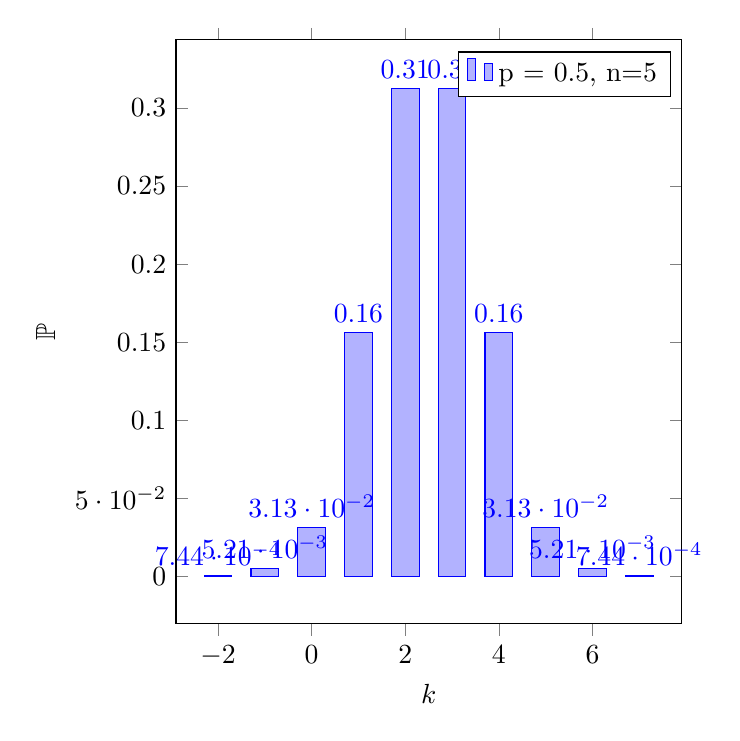
\begin{tikzpicture}[
        declare function={binom(\k,\n,\p)=\n!/(\k!*(\n-\k)!)*\p^\k*(1-\p)^(\n-\k);}
        ]
        \begin{axis}[
            x tick label style={
            /pgf/number format/1000 sep=},
            xlabel=$k$,
            ybar=0,
            ylabel=$\mathbb{P}$,
            width=8cm,
            nodes near coords,
            height=9cm,
                samples at={-2,...,7},
            ]
            \addplot{binom(x,5,0.5)};
            \addlegendentry{p = 0.5, n=5}
        \end{axis}
    \end{tikzpicture}

    % how probably is it that i dont want to keep going to university: 100% :^)
\end{document}
